\documentclass[12pt, handout]{beamer}
\usepackage[polytechnique, psc, complexe, unicouleur]{persobeamer}
%nocouleur ou: unicouleur ou : bicouleur
%complexe ou : simple
%voir dans le package pour changer les couleurs
\usepackage{tikz}

\title{Projet Scientifique collectif INF02}
\subtitle{Soutenance finale}
\author{}
\date{19 mai 2015}


\begin{document}

  \addtobeamertemplate{frametitle}{}{
    \begin{tikzpicture}[remember picture,overlay]
    \node[anchor=south east,yshift=2pt] at (current page.south east) {
\includegraphics[height=0.7cm]{logohori.eps}};

    \end{tikzpicture}
   }

    \begin{frame}
      \maketitle
    \end{frame}		


    %% sommaire %%		
    \begin{frame}
      \frametitle{Sommaire}
      %\tableofcontents[pausesections]
      \tableofcontents
    \end{frame}

%%%%%%%%%%%%%%%%%%%%%%%%
\section{Introduction}
%%%%%%%%%%%%%%%%%%%%%%%%%%

%%%%%%%%%%%%%%%%
\begin{frame}
 \frametitle{But du projet}
 

\end{frame}

%%%%%%%%%%%%%%%%%%%
\begin{frame}
 \frametitle{Modules}
 
 
\end{frame}


\begin{frame}
 \frametitle{Outils extérieurs et points techniques}
 
 
\end{frame}

%%je pense qu'on peut franchement réduire l'état de l'art,
%% à un bref rappel.
%ce n'est pas ce qu'ils veulent entendre à une soutenance

\subsection{État de l'art}

\begin{frame}
 \frametitle{Traitement du langage naturel}
 
 
\end{frame}

\begin{frame}
 \frametitle{\textit{Extractive summarization}}
 
 
\end{frame}

\begin{frame}
 \frametitle{\textit{Abstractive summarization}}
 
 
\end{frame}


\begin{frame}
 \frametitle{Génération du résumé et évaluation}
 
 
\end{frame}

%je vire copycat/bascet, on détaillera mieux
%%sur le RC lui-même

\section{Sources de données}

%\subsection{Données textuelles}

\begin{frame}
 \frametitle{Données textuelles}
 
 
\end{frame}

%\subsection{Données conceptuelles}

\begin{frame}
 \frametitle{Extraction de concepts}
 
 
\end{frame}

\begin{frame}
 \frametitle{WordNet}
 
 
\end{frame}

\begin{frame}
 \frametitle{Conceptnet5}
 
 
\end{frame}

\begin{frame}
 \frametitle{Freebase}
 
 
\end{frame}


%%%%%%%%%%%%%%%%%%%%%%%%%%%
\section{Réseau de concepts}
%%%%%%%%%%%%%%%%%%%%%%%%%%%
% Schrotty !

\subsection{Structure}

\begin{frame}
 \frametitle{Objectifs et utilité du réseau}
 
 \begin{itemize}
  \item Représenter des données conceptuelles ;
  \item Établir des relations sémantiques ;
  \item Fournir des informations de contexte.
 \end{itemize}
 
 Le réseau n'effectue pas la \textbf{sélection} de l'information, mais il en ajoute.
 
\end{frame}


\begin{frame}[allowframebreaks = 0.7, fragile]
 \frametitle{Structure statique du réseau}
 
\begin{block}{N\oe uds}
\begin{itemize}
 \item Étiquette : concept ;
 \item Importance conceptuelle ;
 \item Activation ;
\end{itemize}

\textbf{Exemple :} ["hyperactivity", "ic": 34, "a": 10].

\end{block}
 
\begin{block}{Arêtes}
 \begin{itemize}
  \item Orientées ;
  \item Proximité ;
  \item Relation.
 \end{itemize}

\textbf{Exemple :} ["hyperactivity", "disorder", \{"r": "IsA", "w": 47\}].
 
\end{block}

 
\end{frame}

%%%%%%%%%%%%%%%%%%%%%%%%%%%%%%%%%%%%%%%
\begin{frame}[fragile]
 \frametitle{Propriétés dynamiques du réseau}
 
 \begin{itemize}
  \item  L'activation d'un n\oe ud se propage à ses fils ;
  \item Les n\oe uds se désactivent naturellement.
 \end{itemize}
 
 \textbf{Exemple 1 :} en partant de \verb|"wayne_rooney"| et  \verb|"manchester_united_f.c."|.
 
 \textbf{Exemple 2 :} en considérant les n\oe uds fortement activés (plus de 10\%).
 
 \note{Sur ce premier exemple, on ne montre pas le degré d'activation de chaque noeud, c'est juste pour voir la propagation. Sur le deuxième on s'intéresse déjà plus à la pertinence.}
 
\end{frame}


%%%%%%%%%%%%%%%%%%%%%%%%%%%%%%%
\begin{frame}
  \frametitle{Exemple 1}
% 
%    \begin{overprint}
% \onslide<1> Étape 0 : 2    n\oe uds activés.
% \onslide<2> Étape 1 : 6   n\oe uds activés.
% \onslide<3> Étape 2 : 67   n\oe uds activés.
% \onslide<4> Étape 3 : 51   n\oe uds activés.
% \onslide<5> Étape 4 : 59   n\oe uds activés.
% \onslide<6> Étape 5 : 133   n\oe uds activés.
% \end{overprint}
%   
%   \begin{overlayarea}{8cm}{8cm}
%    \only<1>{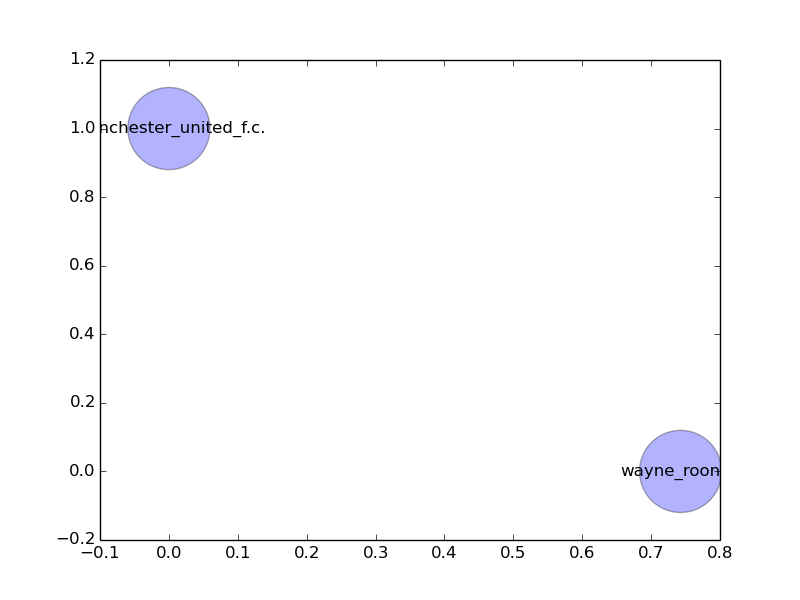
\includegraphics[height=7cm]{examples/touslesnoeuds/0.png}}
%    \only<2>{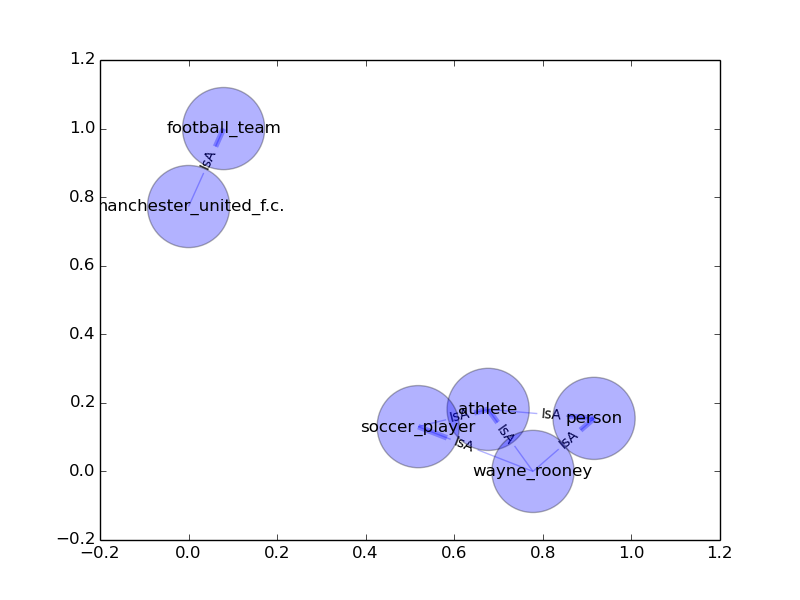
\includegraphics[height=7cm]{examples/touslesnoeuds/1.png}}
%    \only<3>{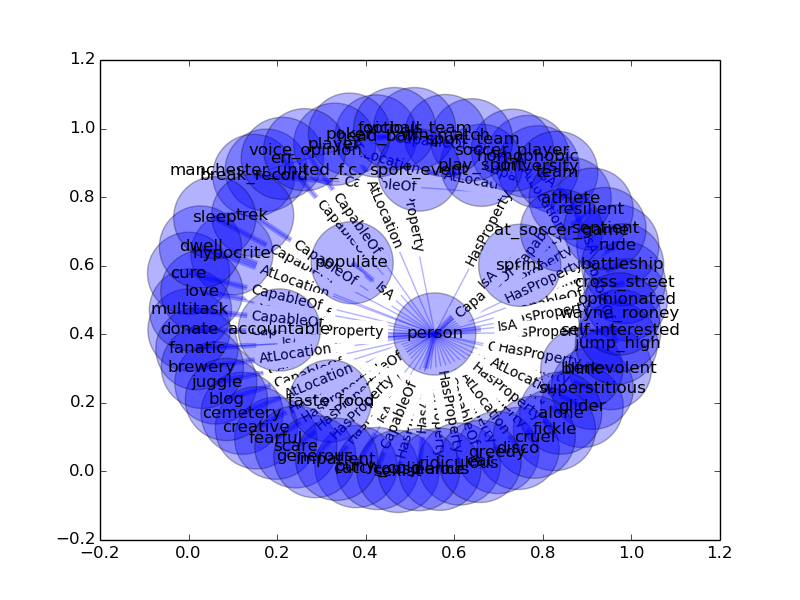
\includegraphics[height=7cm]{examples/touslesnoeuds/2.png}}
%    \only<4>{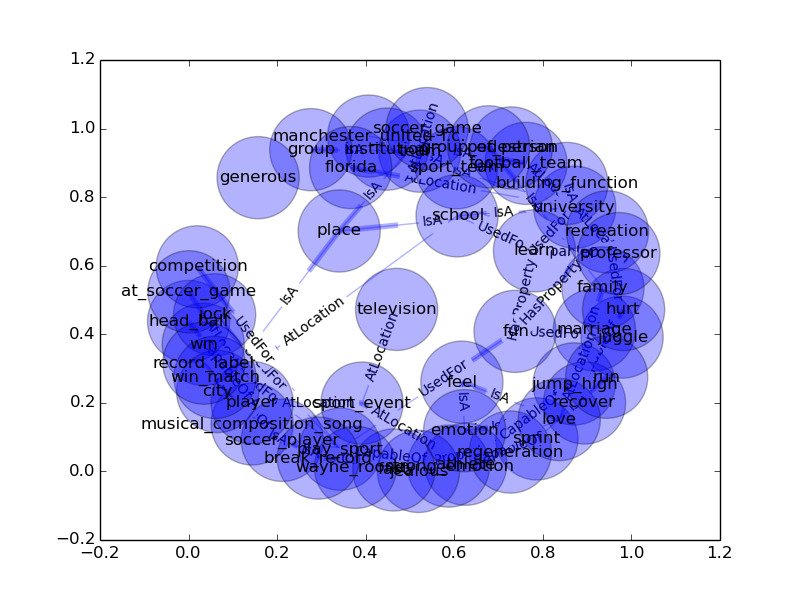
\includegraphics[height=7cm]{examples/touslesnoeuds/3.png}}
%    \only<5>{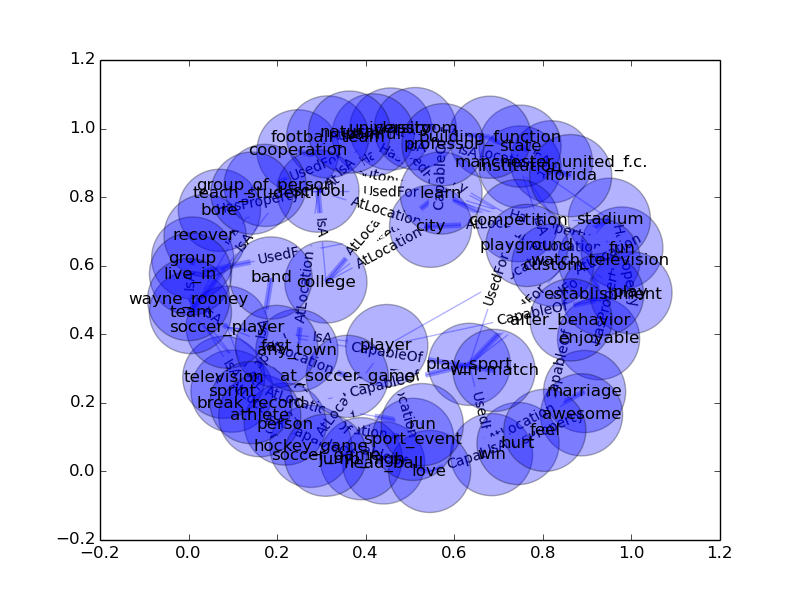
\includegraphics[height=7cm]{examples/touslesnoeuds/4.png}}
%    \only<6>{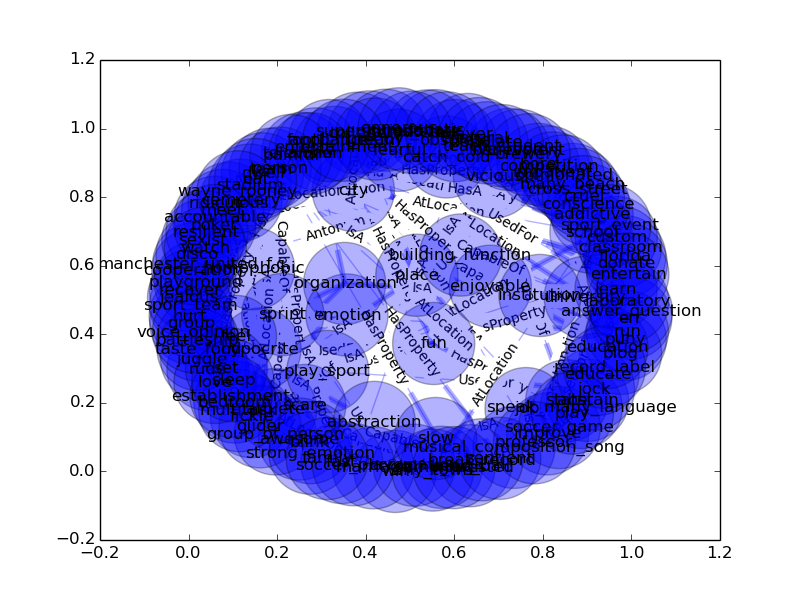
\includegraphics[height=7cm]{examples/touslesnoeuds/5.png}}
%    \only<7>{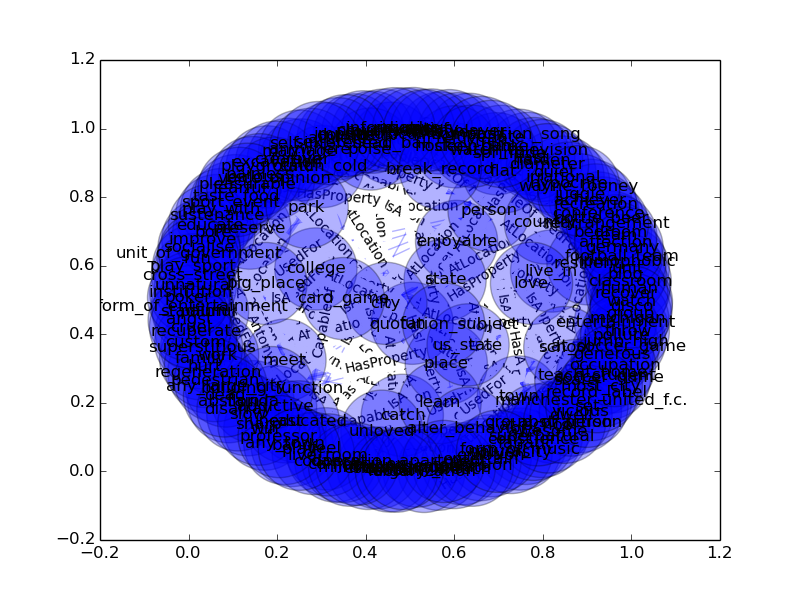
\includegraphics[height=7cm]{examples/touslesnoeuds/6.png}}
%   \end{overlayarea}

\end{frame}

%%%%%%%%%%%%%%%%%%%
\begin{frame}
  \frametitle{Exemple 2}
% 
%    \begin{overprint}
% \onslide<1> Étape 0 : 2    n\oe uds activés.
% \onslide<2> Étape 1 : 3    n\oe uds activés.
% \onslide<3> Étape 2 : 4    n\oe uds activés.
% \onslide<4> Étape 3 : 4   n\oe uds activés.
% \onslide<5> Étape 4 : 5   n\oe uds activés.
% \onslide<6> Étape 5 : 9   n\oe uds activés.
% \onslide<7> Étape 6 : 16   n\oe uds activés.
% \onslide<8> Étape 7 : 22   n\oe uds activés.
% \onslide<9> Étape 8 : 34   n\oe uds activés.
% \onslide<10> Étape 9 : 54   n\oe uds activés.
% \end{overprint}
% 
%   
%   \begin{overlayarea}{8cm}{8cm}
%    \only<1>{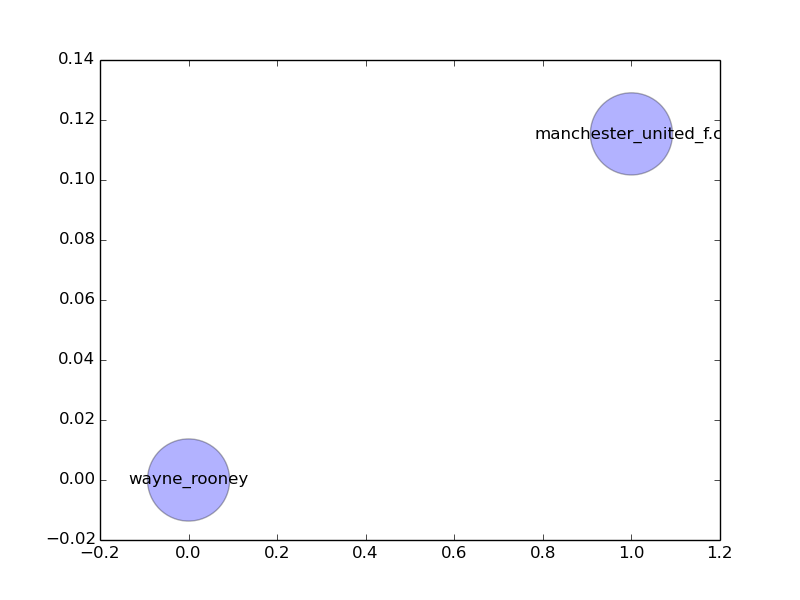
\includegraphics[height=7cm]{examples/noeudsbienactives/0.png}}
%    \only<2>{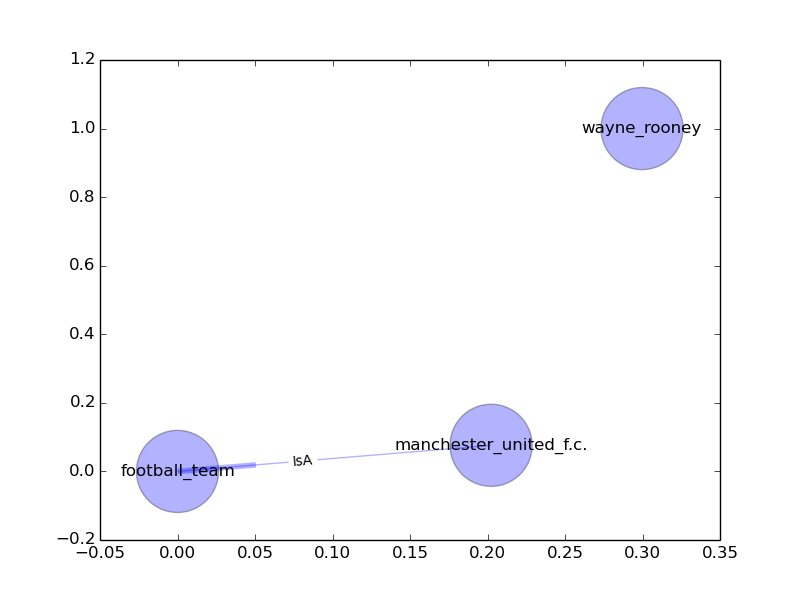
\includegraphics[height=7cm]{examples/noeudsbienactives/1.png}}
%    \only<3>{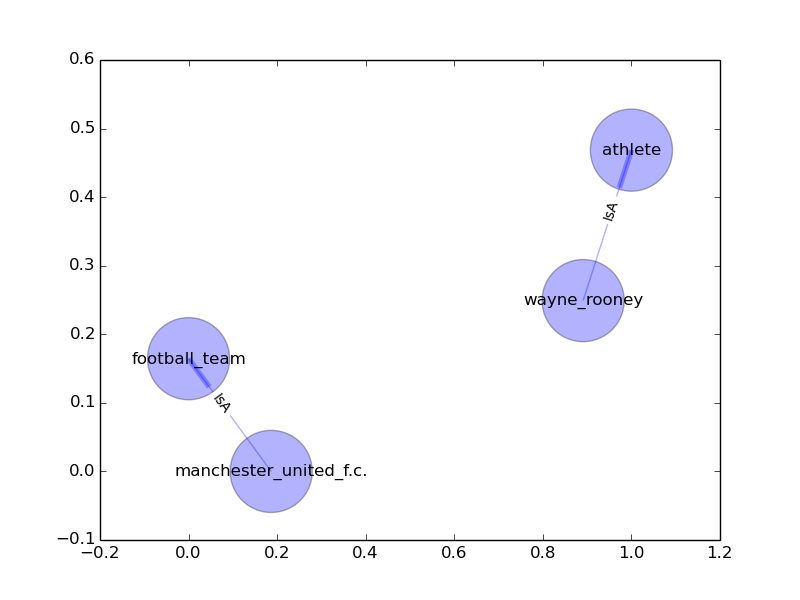
\includegraphics[height=7cm]{examples/noeudsbienactives/2.png}}
%    \only<4>{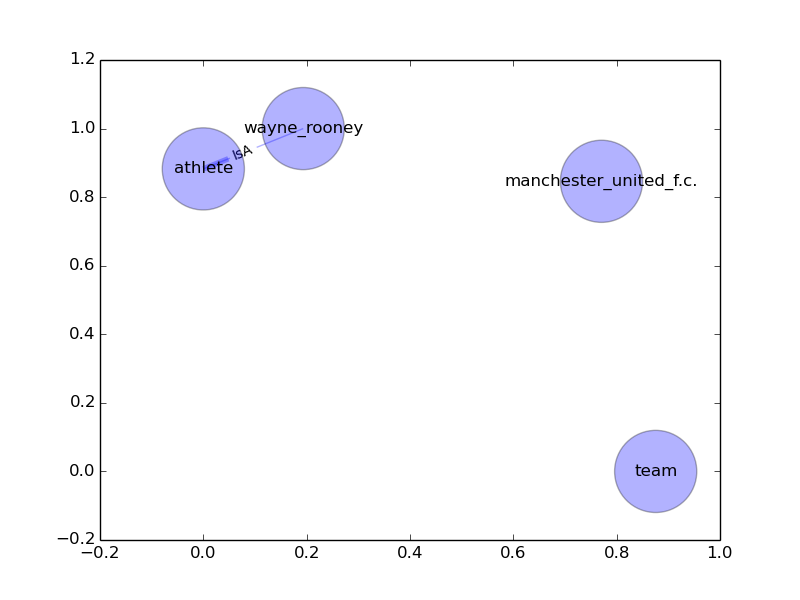
\includegraphics[height=7cm]{examples/noeudsbienactives/3.png}}
%    \only<5>{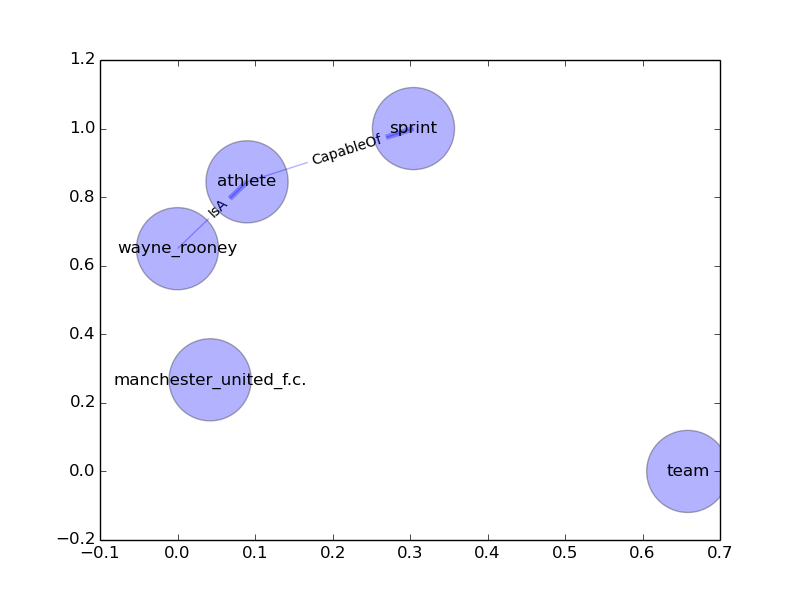
\includegraphics[height=7cm]{examples/noeudsbienactives/4.png}}
%    \only<6>{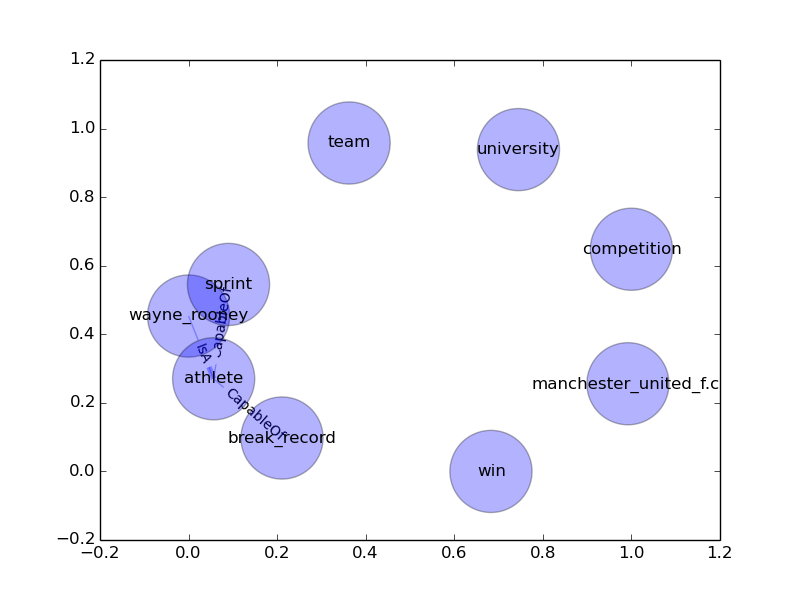
\includegraphics[height=7cm]{examples/noeudsbienactives/5.png}}
%    \only<7>{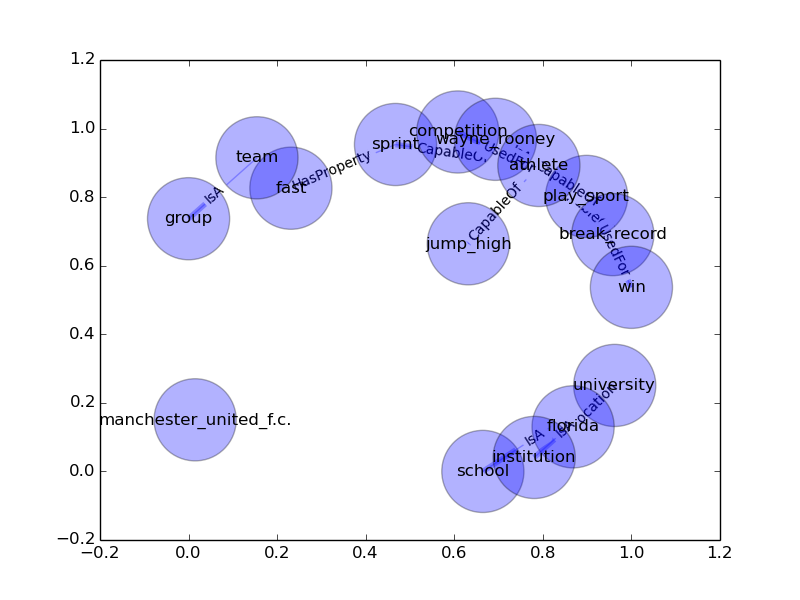
\includegraphics[height=7cm]{examples/noeudsbienactives/6.png}}
%    \only<8>{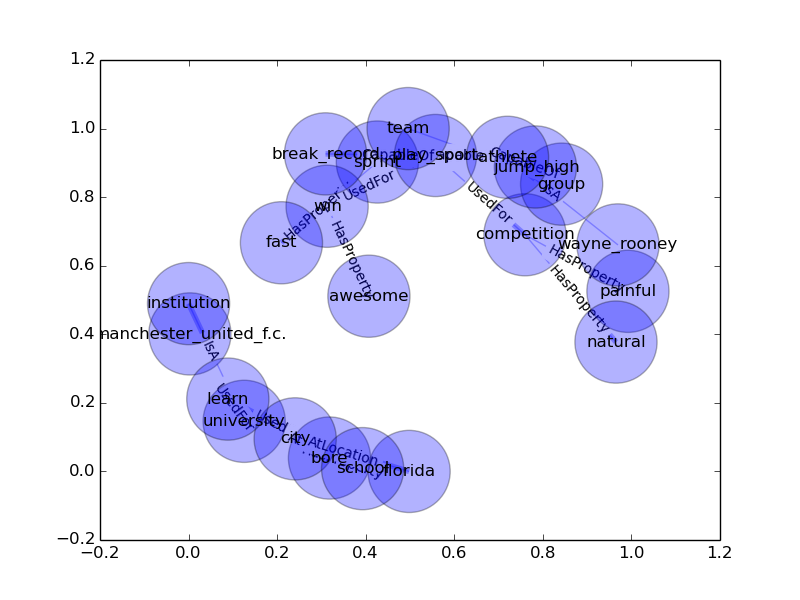
\includegraphics[height=7cm]{examples/noeudsbienactives/7.png}}
%    \only<9>{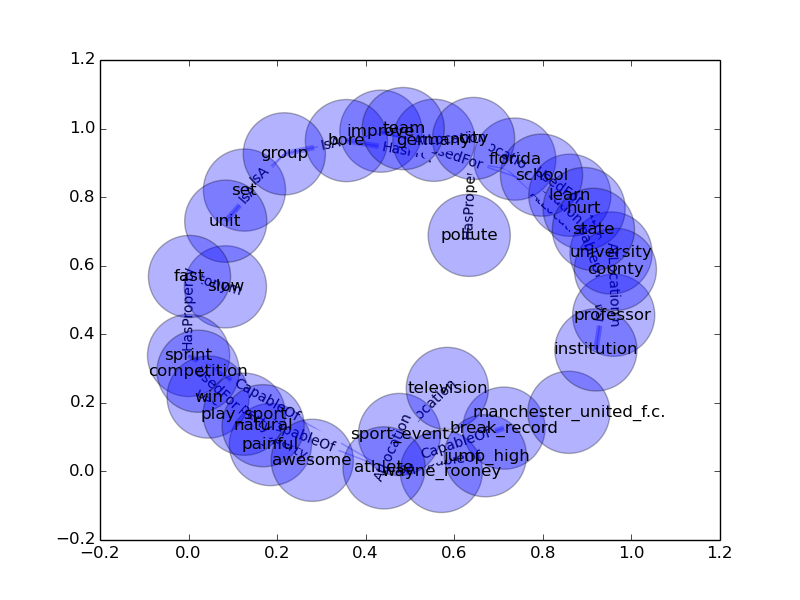
\includegraphics[height=7cm]{examples/noeudsbienactives/8.png}}
%    \only<10>{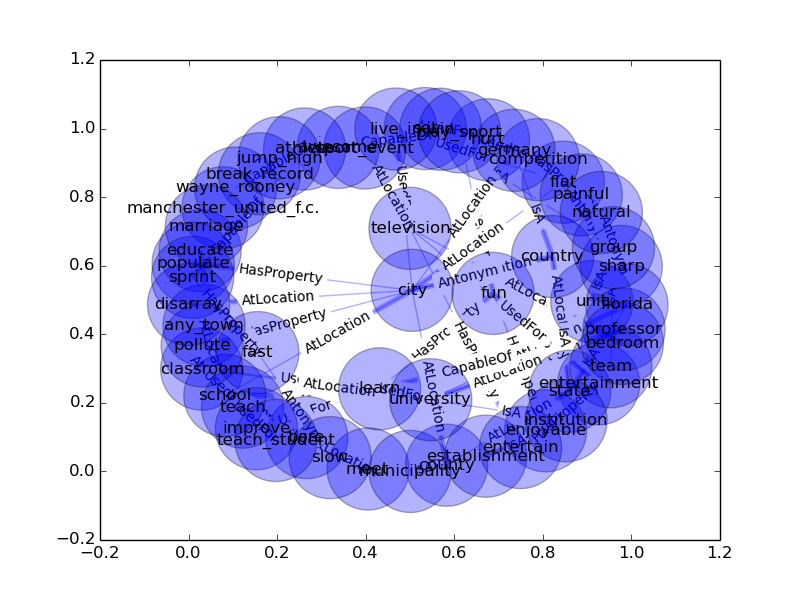
\includegraphics[height=7cm]{examples/noeudsbienactives/9.png}}
%   \end{overlayarea}

\end{frame}


%%%%%%%%%%%%%%%%%%%%%%%%%%%%%%%
\begin{frame}
 \frametitle{Détails}
 
 \begin{itemize}
  \item Les concepts "font penser" à d'autres concepts : \textbf{contexte} ;
  \item Certains concepts sont oubliés : \textbf{sélection}.
 \end{itemize}

 On ne cherche pas un état d'équilibre. Il faut tirer parti de ces deux propriétés en réglant le nombre d'étapes.
 
\end{frame}

\begin{frame}
  \frametitle{Désactivation}
 
 \begin{block}{Comment désactiver ?}
 \begin{itemize}
  \item En fonction de l'importance conceptuelle ;
  \item En fonction du nombre de liens.
  \end{itemize}
 \end{block}

 \textbf{Exemple 3 :}  N\oe uds bien activés, sans tenir compte du nombre de liens.
 
 \textbf{Exemple 4 :} En introduisant maintenant une dépendance du nombre de liens.
 
 \note{!!!! Pour l'importance conceptuelle, on verra plus tard avec les méthodes statistiques. Grosso modo, plus un noeud est important, moins vite il se désactive. Pour l'exemple 3, même exemple que le deuxième, mais avec cette fois un facteur log égal à 1, donc aucune dépendance avec le nombre de liens.}
 
 \note{Exemple pathologique : un mot comme "<water"> a 44 voisins avec de bons poids}
 
\end{frame}


%%%%%%%%%%%%%%%%%%%%%%%%%%%%%%%%%
\begin{frame}
\frametitle{Exemple 3}

%     \begin{overprint}
%       \onslide<1> Étape 0 : 2  n\oe uds activés.
%       \onslide<2> Étape 1 : 5  n\oe uds activés.
%       \onslide<3> Étape 2 : 14 n\oe uds activés.
%       \onslide<4> Étape 3 : 26 n\oe uds activés.
%       \onslide<5> Étape 4 : 51 n\oe uds activés.
%       \onslide<6> Étape 5 : 114 n\oe uds activés.
%       \onslide<7> Étape 6 : 209 n\oe uds activés.
%       \onslide<8> Étape 7 : 334 n\oe uds activés.
%     \end{overprint} 
% 
%   
%   \begin{overlayarea}{8cm}{8cm}
%    \only<1>{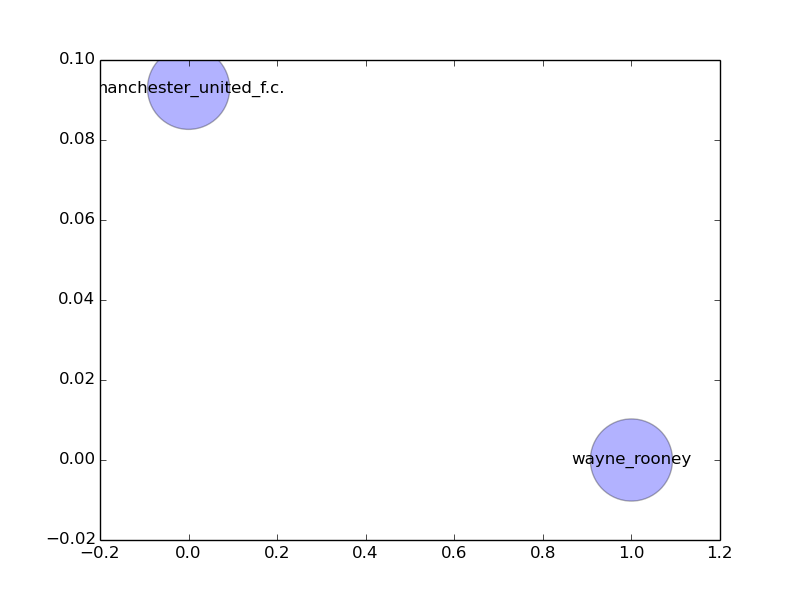
\includegraphics[height=7cm]{examples/facteurlogun/0.png}}
%    \only<2>{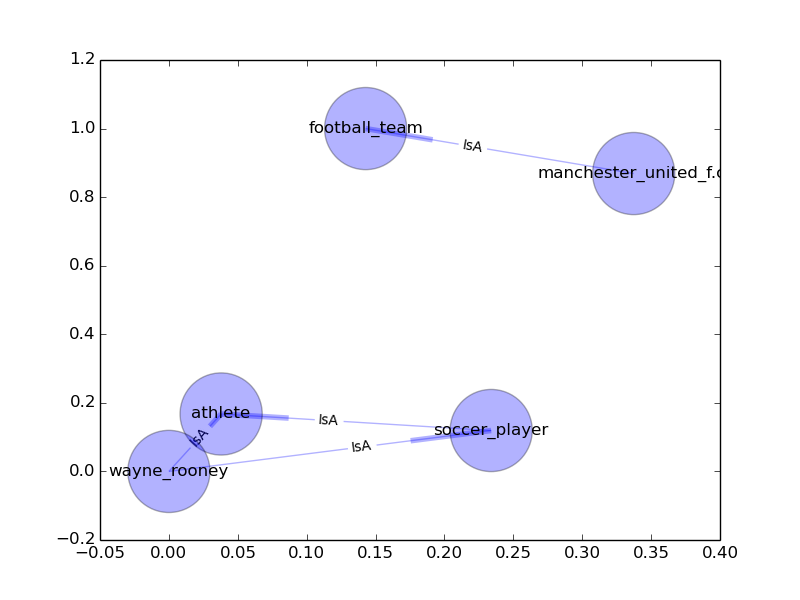
\includegraphics[height=7cm]{examples/facteurlogun/1.png}}
%    \only<3>{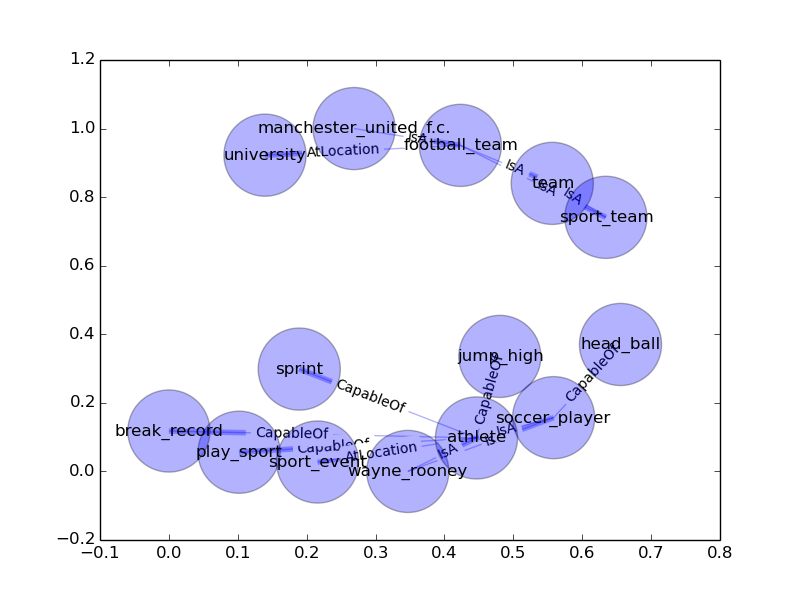
\includegraphics[height=7cm]{examples/facteurlogun/2.png}}
%    \only<4>{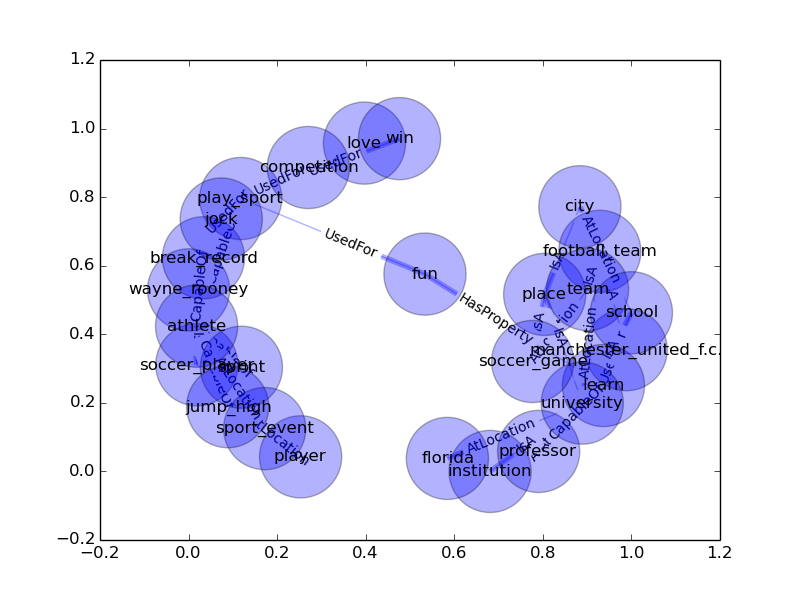
\includegraphics[height=7cm]{examples/facteurlogun/3.png}}
%    \only<5>{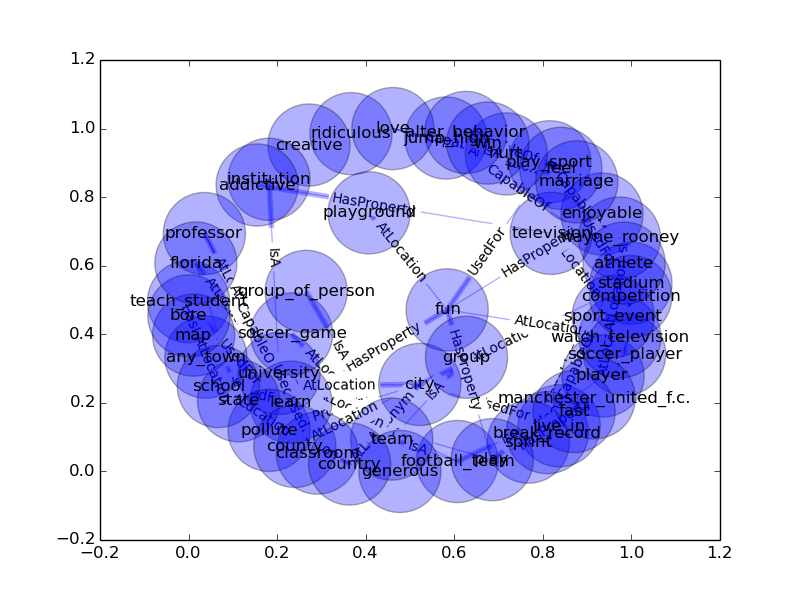
\includegraphics[height=7cm]{examples/facteurlogun/4.png}}
%    \only<6>{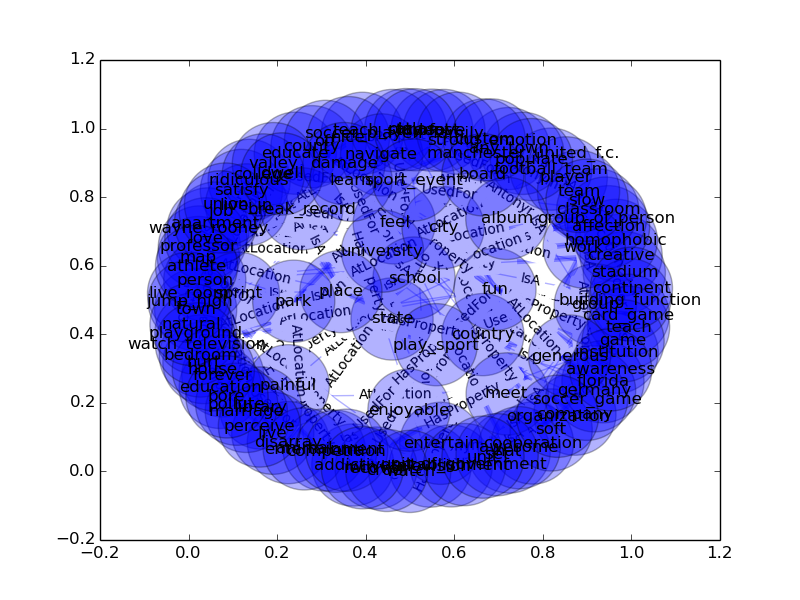
\includegraphics[height=7cm]{examples/facteurlogun/5.png}}
%    \only<7>{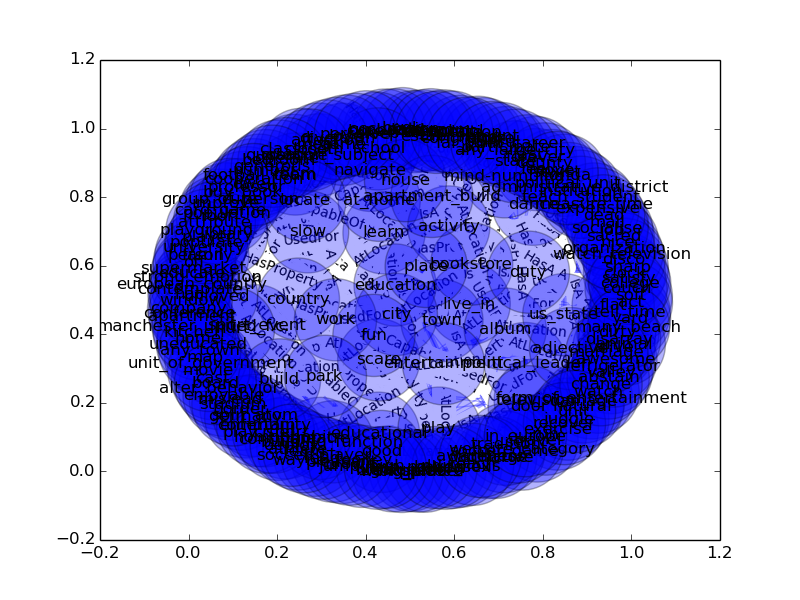
\includegraphics[height=7cm]{examples/facteurlogun/6.png}}
%    \only<8>{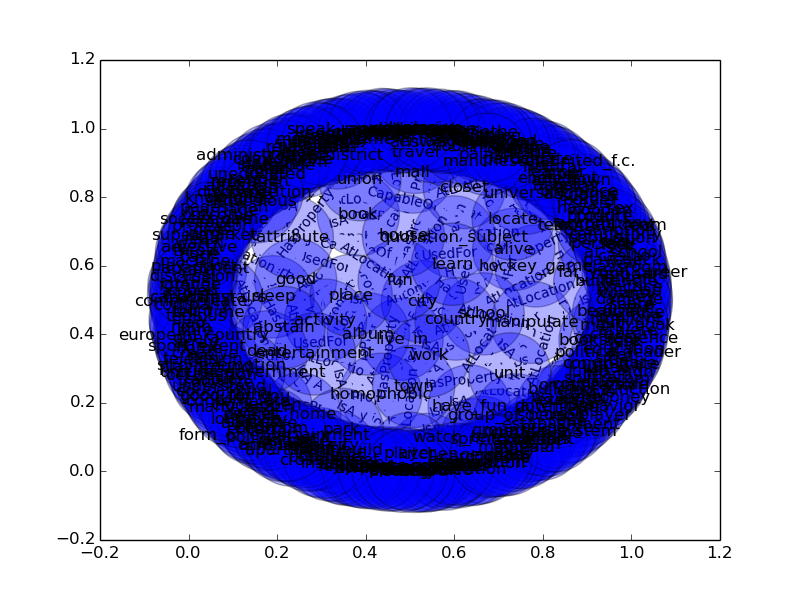
\includegraphics[height=7cm]{examples/facteurlogun/7.png}}
%   \end{overlayarea}

\end{frame}

%%%%%%%%%%%%%%%%%%%%%%%%%%%
\begin{frame}
 \frametitle{Exemple 4}
 
%     \begin{overprint}
%       \onslide<1> Étape 0 : 2  n\oe uds activés.
%       \onslide<2> Étape 1 : 3   n\oe uds activés.
%       \onslide<3> Étape 2 : 2  n\oe uds activés.
%       \onslide<4> Étape 3 : 3  n\oe uds activés.
%       \onslide<5> Étape 4 : 3  n\oe uds activés.
%       \onslide<6> Étape 5 : 4  n\oe uds activés.
%       \onslide<7> Étape 6 : 6  n\oe uds activés.
%       \onslide<8> Étape 7 : 9  n\oe uds activés.
%     \end{overprint} 
% 
%   
%   \begin{overlayarea}{8cm}{8cm}
%    \only<1>{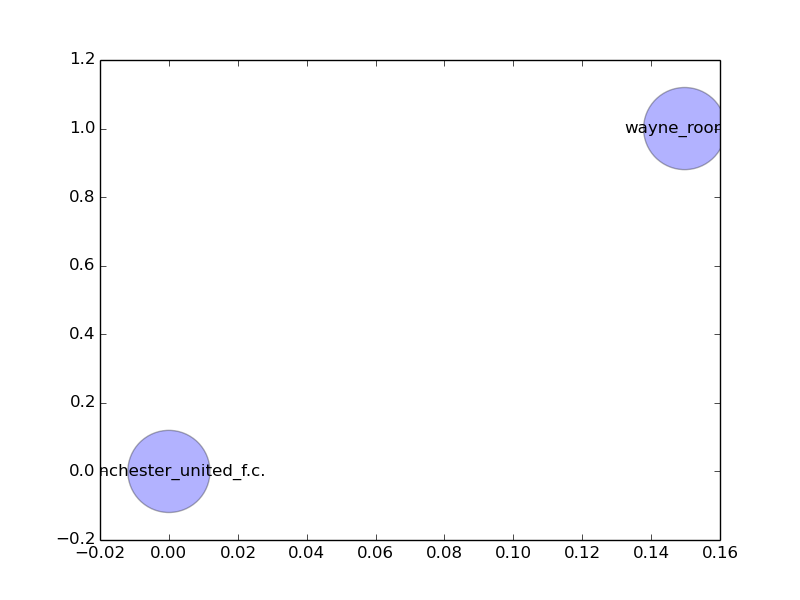
\includegraphics[height=7cm]{examples/grosfacteurlog/0.png}}
%    \only<2>{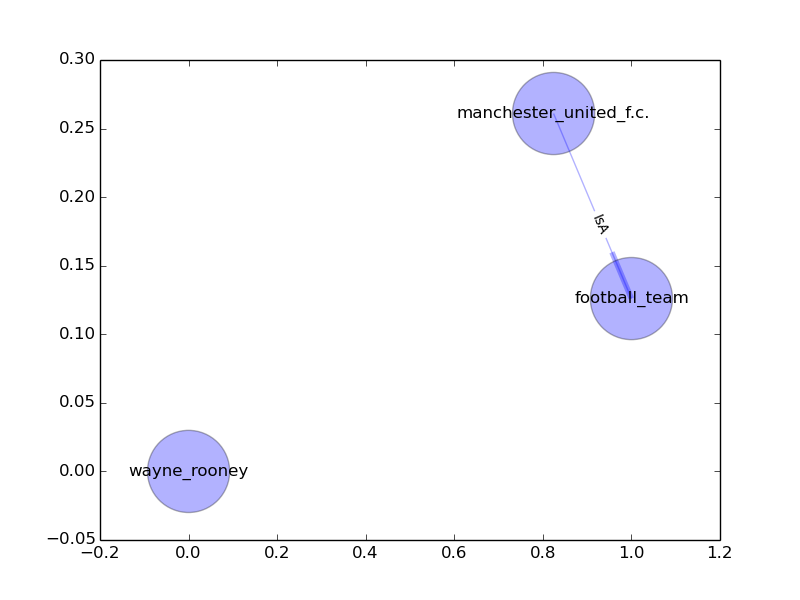
\includegraphics[height=7cm]{examples/grosfacteurlog/1.png}}
%    \only<3>{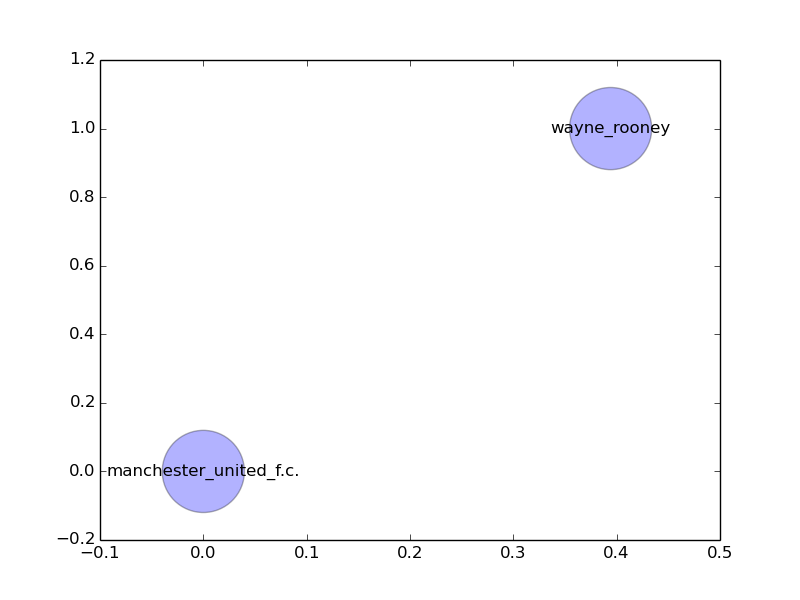
\includegraphics[height=7cm]{examples/grosfacteurlog/2.png}}
%    \only<4>{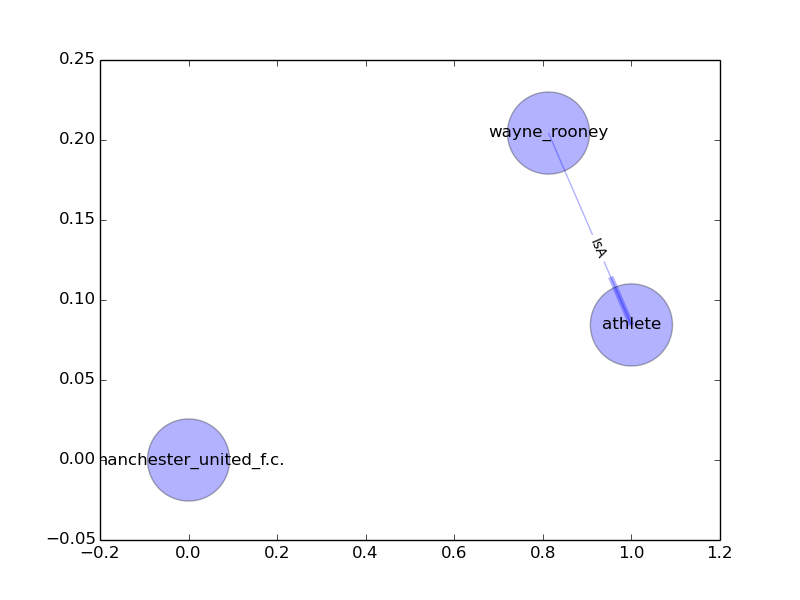
\includegraphics[height=7cm]{examples/grosfacteurlog/3.png}}
%    \only<5>{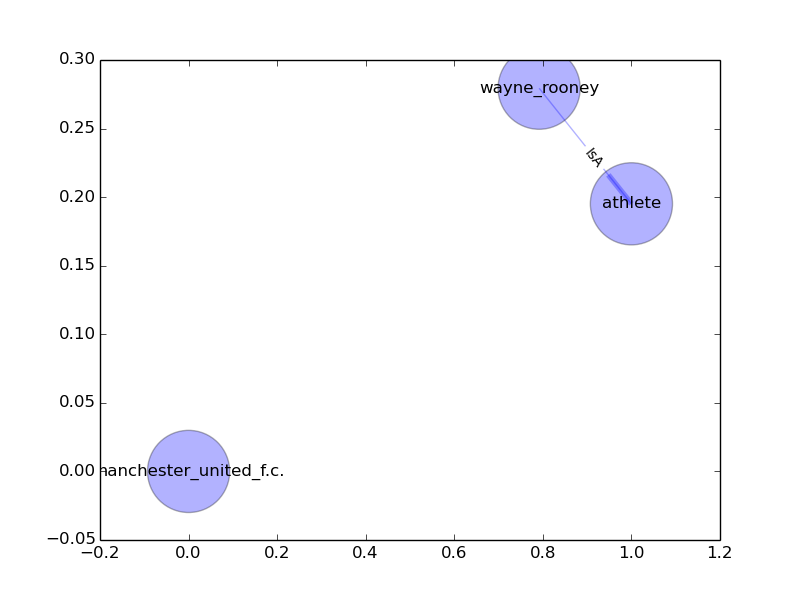
\includegraphics[height=7cm]{examples/grosfacteurlog/4.png}}
%    \only<6>{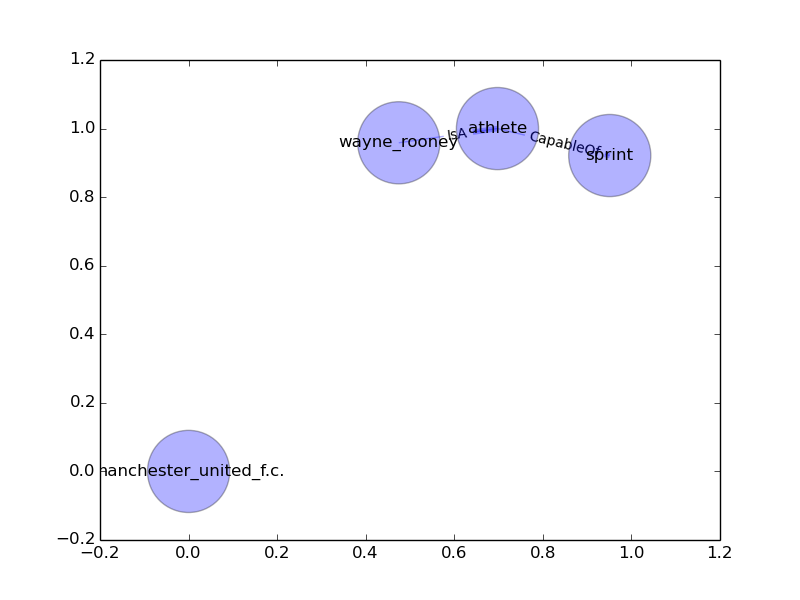
\includegraphics[height=7cm]{examples/grosfacteurlog/5.png}}
%    \only<7>{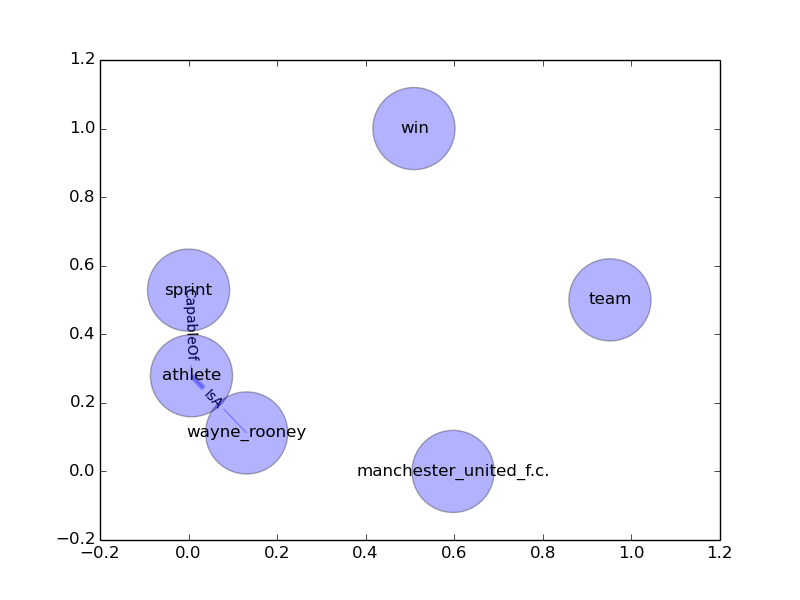
\includegraphics[height=7cm]{examples/grosfacteurlog/6.png}}
%    \only<8>{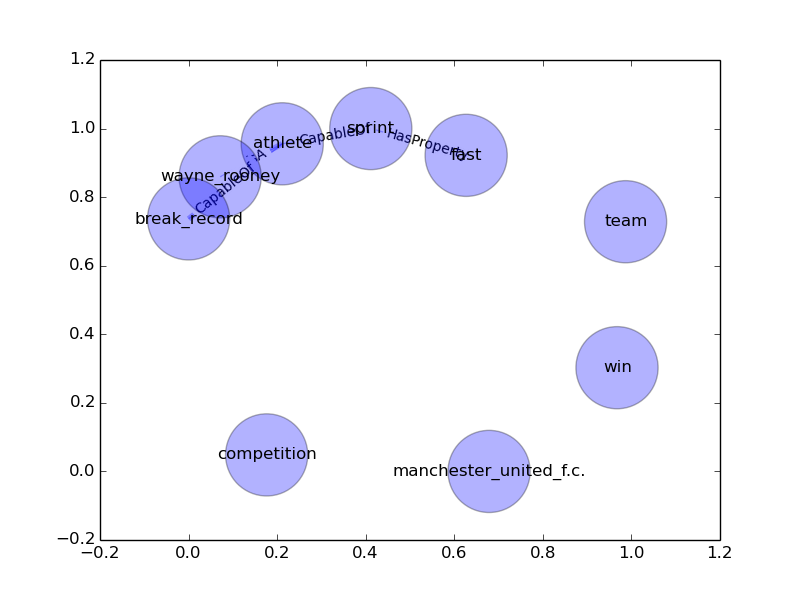
\includegraphics[height=7cm]{examples/grosfacteurlog/7.png}}
%   \end{overlayarea}

\end{frame}



%%%%%%%%%%%%%%%%%%%%%%%%%
\subsection{Construction}
%%%%%%%%%%%%%%%%%%%%%%%%

%%%%%%%%%%%%%%%%%%%%%%%%%%ù
\begin{frame}
 \frametitle{Construction du réseau}
 
 Récupération de listes :
 
 \begin{itemize}
  \item De concepts (noms communs, verbes...) ;
  \item De noms propres.
 \end{itemize}

 \pause
 
 Lancement de requêtes :
 \begin{itemize}
  \item Conceptnet5 ;
  \item Freebase.
 \end{itemize}
 
 \pause
 
 Extension à partir des premiers n\oe uds, par d'autres requêtes.
 
 \note{Nous partons de texte brut, digéré avec différents outils.}
 
\end{frame}

%%%%%%%%%%%%%%
\begin{frame}
  \frametitle{Exemple obtenu}
  
  \begin{itemize}
   \item Plus de 18~000 noms propres et concepts comme base (ayant donné des résultats positifs lors des requêtes) ;
   \item Extension à plus de 28~000 n\oe uds bien reliés entre eux ;
   \item Plus de 16~000 n\oe uds sans lien entrant.
  \end{itemize}

\note{Les noeuds sans lien entrant ne seront pas activés si on ne les trouve pas tels quels dans un texte.}
  
\end{frame}

%%%%%%%%%%%%%%%%%%%%
\begin{frame}[fragile]
 \frametitle{Exemple obtenu}
 
 \begin{block}{Meilleurs en liens sortants}
  \begin{verbatim}
human : 41
water : 44
person : 50
someone : 161
something : 192 
  \end{verbatim}
 \end{block}

  \begin{block}{Meilleurs en liens entrants}
    \begin{verbatim}
soccer_player : 1931
soccer_midfielder : 1575
athlete : 2182
person : 3469
organisation, country...
    \end{verbatim}
  \end{block}
\end{frame}


%%optionnel, et même beaucoup trop chiant
\begin{frame}
 \frametitle{Choix de programmation}
 
 
\end{frame}



\section{TF-IDF et méthodes statistiques}


\begin{frame}
 \frametitle{Définition de l'indice TF-IDF}
 \begin{itemize}
  \item TF: fréquence d'un terme ;
  \item IDF: fréquence inverse de document ;
  \item TF-IDF et poids d'une phrase.
 \end{itemize}
 
\end{frame}

\begin{frame}
 \frametitle{TF-IDF pour résumer}
 \begin{itemize}
  \item Algorithme;
  	\begin{itemize}
  	\item Cacule de poids
  	\item Extraction de phrases
  	\end{itemize}
  \item Qualité de résumé.
 \end{itemize}
 
\end{frame}


\begin{frame}
 \frametitle{TF-IDF pour l'importance conceptuelle}
 \begin{itemize}
  	\item Qeulques charactères de l'importance conceptuelle
  	\item Le cacule adapté
  \end{itemize}
 
\end{frame}


\section{Traitement préalable des données}

%%\subsection{Analyse syntaxique}

\begin{frame}
 \frametitle{Grammaires}
 
 
\end{frame}

\begin{frame}
 \frametitle{État du texte en fin d'analyse}
 
 
\end{frame}


\begin{frame}[allowframebreaks = 0.7]
 \frametitle{Résolution de pronoms}
 
 
\end{frame}


\section{Traitement du réseau}

\subsection{Workspace}

\begin{frame}
 \frametitle{Workspace}
 
 
\end{frame}

\begin{frame}
 \frametitle{}
 
 
\end{frame}

\subsection{Algorithme final}

\begin{frame}
 \frametitle{Algorithme final}
 
 
\end{frame}

\begin{frame}
 \frametitle{Exemples}
 
 
\end{frame}

\section{Conclusion}

\begin{frame}
 \frametitle{Conclusion}
 
C'était vraiment trop mythe comme PSC.
 
\end{frame}

\end{document}
